%-----------------------------------------------------------------------
%
%   UFRJ  - Universidade Federal do Rio de Janeiro
%   COPPE - Coordena��o dos Programas de P�s-gradua��o em Engenharia
%   PEE   - Programa de Engenharia El�trica
%
%   COE-835  Controle adaptativo
%
%   Relat�rio da simula��o
%                                                         Ramon R. Costa
%                                                         05/out/09, Rio
%-----------------------------------------------------------------------
\documentclass[11pt,a4paper]{article}
\usepackage[latin1]{inputenc} %pacote para utilizar palavras acentuadas
\usepackage{amsmath,amssymb}  %pacotes do AMS
\usepackage{latexsym}         %pacote para incluir s�mbolos (ex.\Box)
\usepackage{fancybox,fancyhdr}%pacote com frescuras
\usepackage{graphicx}         %pacote para incluir figuras tipo eps
\usepackage[portuguese]{babel}
\usepackage{xcolor}
\usepackage{float} 
\usepackage{epstopdf}
\usepackage[inline]{enumitem}
\usepackage[a4paper]{hyperref}% Make sure it comes last of your loaded packages
\hypersetup{
  verbose,
  plainpages=false,
  bookmarks=true,
  colorlinks=true,
  linkcolor=blue
}
 
%Matlab code in latex 
\usepackage[final]{listings}
\usepackage{color} %red, green, blue, yellow, cyan, magenta, black, white
\definecolor{mygreen}{RGB}{28,172,0}
\definecolor{mylilas}{RGB}{170,55,241}
\lstdefinestyle{myMatlab}
{
language=matlab,frame=single, basicstyle=\small\ttfamily,breaklines=true,%
morekeywords={matlab2tikz}, keywordstyle=\color{blue}, morekeywords=[2]{1}, keywordstyle=[2]{\color{black}}, commentstyle=\color{mygreen}, stringstyle=\color{mylilas}, identifierstyle=\color{black}, showstringspaces=false,%without this there will be a symbol in the places where there is a space
numbers=left, numberstyle={\scriptsize \color{black}},% size of the numbers
numbersep=9pt, % this defines how far the numbers are from the text
% emph=[1]{for,end,break},emphstyle=[1]\color{red}, %some words to emphasise
% emph=[2]{word1,word2}, emphstyle=[2]{style},
}
     
%----------------------------------------------------------------------
%
%   Macros utilizados no LATEX
%                                                       Ramon R. Costa
%                                                       13/out/17, Rio
%----------------------------------------------------------------------
\newcount\m
\newcount\n

\def\twodigits#1{\ifnum #1<10 0\fi \number#1}

\def\hours{\n=\time \divide\n 60
    \m=-\n \multiply\m 60 \advance\m \time
    \twodigits\n:\twodigits\m}

\def\hora{\hours}

\def\fim{
  \medskip
  \begin{center}
    \rule[1mm]{30mm}{0.14mm}$\diamond$\rule[1mm]{30mm}{0.14mm}
  \end{center}
}

%----------------------------------------------------------------------
% A4 paper size & margins
\setlength {\textheight}    {25cm}%
\setlength {\textwidth}     {17.5cm}%
\setlength {\parindent}     {0mm}%
\setlength {\parskip}       {1mm}%
\setlength {\topmargin}     {-14mm}%
\setlength {\oddsidemargin} {-6mm}%
\setlength {\evensidemargin}{-6mm}%
\setlength {\columnsep}     {6mm}%

%----------------------------------------------------------------------
\def\codigo{COE-835}
\def\disciplina{Controle adaptativo}
\def\periodo{3o. período/2017}
\def\professor{Ramon}

\newcommand{\BOX}[1]{
  \framebox{{\color{magenta}\rule[-3mm]{1mm}{9mm}} ~~$\displaystyle
  \begin{aligned} #1 \end{aligned}$~~}\pagestyle{plain}
}

\newcommand{\RED}[1]{\colorbox{white}{\textcolor{red}{#1}}}
%\newcommand{\WoR}[1]{\colorbox{red}{\textcolor{white}{#1}}}
\newcommand{\BLU}[1]{\colorbox{white}{\textcolor{blue}{#1}}}
\newcommand{\GRE}[1]{\colorbox{green}{\textcolor{black}{#1}}}
\newcommand{\HI}[1]{\colorbox{yellow}{\textcolor{black}{#1}}}  %% Highlithed text

\newcommand{\estrela}[1]{
  \def\TXT{\RED{$\bigstar$ }}
  \hspace*{5mm}\TXT \hfill
  \parbox[t]{ \textwidth - \widthof{\TXT} - 5mm}{#1}
  \par
}

\def\Ltwo{\mbox{${\mathcal L}_2$}}
\def\Linf{\mbox{${\mathcal L}_\infty$}}

\newcommand{\sign}{\mbox{sign}}

\newcommand{\equacao}[2]{
  \makebox[40mm][l]{#1 \dotfill}: \quad \parbox[t]{8cm}
	{\begin{equation} \displaystyle
  \begin{aligned}
    #2
  \end{aligned} \end{equation}} \\
}

\newcommand{\sref}[1]{Section~\ref{#1}}
\newcommand{\fref}[1]{Fig.~\ref{#1}}
\newcommand{\tref}[1]{Table~\ref{#1}}
\newcommand{\thref}[1]{Theorem~\ref{#1}}
\newcommand{\aref}[1]{Assumption~\ref{#1}}
\newcommand{\norm}[1]{\left\lVert#1\right\rVert}
%\renewcommand{\qedsymbol}{}
\newcommand{\rev}[1]{{\color{red}#1}}
%\newcommand{\mat}[1]{\begin{bmatrix}#1\end{bmatrix}}

\newtheorem{remark}{Remark}
\newtheorem{lemma}{Lema}

%----------------------------------------------------------------------


%Set normal paragraph spacing
\setlength\parindent{24pt}

\begin{document}
%---------------------------------------------------------------------
\pagestyle{fancy}%
\renewcommand{\headrulewidth}  {0.4pt}%
\renewcommand{\footrulewidth}  {0.4pt}%
\lhead{\bfseries{Relat�rio do Trabalho 10}}%
\chead{}%
\rhead{\bfseries\thepage}%
\lfoot{}%
\cfoot{}%
\rfoot{[\hours] \quad \today}%
%---------------------------------------------------------------------
\begin{center}
  \huge{COE-835  Controle  adaptativo}  \\[20mm]

  \Large{Trabalho 10} \\[20mm]
\end{center}

\textbf{Grupo:} \quad \parbox[t]{10cm}{
Guilherme Pires Sales de Carvalho \\[2mm]
Matheus Ferreira dos Reis \\[2mm]
Renan Salles de Freitas \\[10mm]
}

\textbf{Algoritmo:} \quad \HI{Adaptive Backstepping Control}\\[2mm]

\bigskip%
\textbf{Caso}: \quad \parbox[t]{10cm}{
  $n = 3$ \quad (ordem da planta) \\[2mm]
  $n^* = 3$ \quad (grau relativo) \\[2mm]
  $n_p = 4$ \quad (\# de par�metros) \\[15mm]
}

%---------------------------------------------------------------------
\tableofcontents
\newpage
%---------------------------------------------------------------------
%---------------------------------------------------------------------
\section{Backstepping - Formula��o te�rica sem observador}

Backstepping � um m�todo recursivo de controle adaptativo baseado em Lyapunov e
proposto no come�o da d�cada de 90. A ideia � projetar um controle recursivo
considerando algumas das vari�veis de estado como ``controle virtuais'' e
implementar para elas leis de controle intermedi�rias. Com esta t�cnica �
poss�vel resolver problemas de estabilidade e rastreamento. Neste trabalho,
desenvolveremos a fundamenta��o te�rica para o caso de um sistema de
segunda ordem com par�metros desconhecidos:

\begin{align}
\dot{x}_1 &= x_2 + \phi_1^\intercal(x_1) \, \theta\\
\nonumber \dot{x}_2 &= k_p\,u + \phi_2^\intercal(x_1,x_2)\,\theta
\label{eq:planta}
\end{align}

onde $\theta$ � o vetor de par�metros desconhecidos e $k_p$ � o ganho de
alta frequ�ncia, tamb�m desconhecido. As n�o linearidades do sistema s�o
representadas pela vari�vel $\phi$. Para o desenvolvimento do algoritmo,
assume-se:

\begin{itemize}
  \item o sinal de $k_p$ � conhecido;
  \item o sinal de refer�ncia $y_r$ e suas derivadas s�o cont�nuas e limitadas.
\end{itemize}

Introduzem-se as vari�veis $\textbf{z}$ (mudan�a de coordenadas):

\begin{align}
z_1 &= x_1 - y_r \\
\nonumber z_2 &= x_2 - \alpha_1 - \dot{y}_r,
\end{align}

onde $\alpha$ � a vari�vel de controle virtual. O primeiro passo para a
elabora��o do m�todo � come�ar pela equa��o \ref{eq:planta},
considerando $x_2$ como uma vari�vel de controle virtual. A derivada do erro de
rastreamento $z_1$ � dada por:

\begin{align}
\dot{z}_1 &= \dot{x}_1 - \dot{y}_r \\
\nonumber &= z_2 + \alpha_1 + \phi_1^\intercal\,\theta
\end{align}

Podemos projetar a primeira fun��o estabilizante $\alpha_1$ como:

\begin{equation}
\alpha_1 = -c_1z_1 - \phi_1^\intercal\,\hat{\theta},
\end{equation}

onde $c_1$ � uma constante positiva e $\hat{\theta}$ � uma estimativa de
$\theta$. Consideremos a fun��o de Lyapunov:

\begin{equation}
V_1 = \frac{1}{2}z_1^2 +
\frac{1}{2}\tilde{\theta}^\intercal\,\Gamma^{-1}\,\tilde{\theta},
\end{equation}

onde $\Gamma$ � uma matriz positiva definida e
$\tilde{\theta}=\theta-\hat{\theta}$. Derivando a fun��o de Lyapunov, temos:

\begin{align}
\dot{V}_1 &= z_1\dot{z}_1 -
\tilde{\theta}^\intercal\,\Gamma^{-1}\,\dot{\hat{\theta}}\\
\nonumber &=
z_1(z_2+\alpha_1+\phi_1^\intercal
\, \hat{\theta})-\tilde{\theta}^\intercal(\Gamma^{-1} \,
\dot{\hat{\theta}}-\phi_1z_1)\\
\nonumber &= -c_1z_1^2+\tilde{\theta}^\intercal(\tau_1-\Gamma^{-1} \,
\dot{\hat{\theta}}) + z_1z_2\\
\tau_1 &= \phi_1z_1
\end{align}

Observe que se escolhermos a varia��o dos par�metros como
$\dot{\hat{\theta}}=\Gamma\,\tau_1$ anulamos um dos termos, mas ainda falta
considerar a din�mica de $z_2$. Devemos deixar a escolha da lei de adapta��o em
aberto. Pela segunda equa��o, temos:
 
\begin{align}
\dot{z}_2 &= k_pu + \phi_2^\intercal \, \theta - \dot{\alpha_1}-\ddot{y}_r \\
\nonumber &= k_pu + \phi_2^\intercal \, \theta -
\frac{\partial\alpha_1}{\partial x_1}(x_2 + \phi_1^\intercal \, \theta) -
\frac{\partial\alpha_1}{\partial \hat{\theta}}\dot{\hat{\theta}} -
\frac{\partial\alpha_1}{\partial y_r}\dot{y}_r - \ddot{y}_r
\end{align}

Escolhemos a fun��o Lyapunov:

\begin{align}
V = V_1 + \frac{1}{2}z_2^2 + \frac{|k_p|}{2\gamma}\tilde{p}^2, 
\end{align}

onde $\tilde{p}=p-\hat{p}$ e $\hat{p}$ � estimativa de $p = \frac{1}{k_p}$, e
$\gamma > 0$. Derivando a fun��o Lyapunov, obtemos:

\begin{align}
\dot{V} &= -c_1z_1^2 + z_1z_2 +
\tilde{\theta}^\intercal(\tau_1-\Gamma^{-1}\dot{\hat{\theta}}) + z_2\dot{z}_2 +
\frac{|k_p|}{\gamma}\tilde{p}\dot{\tilde{p}} \notag\\
\nonumber &= -c_1z_1^2 + z_1z_2 +
\tilde{\theta}^\intercal(\tau_1-\Gamma^{-1}\dot{\hat{\theta}}) + z_2\left( k_pu
+ \phi_2^\intercal \, \theta - \frac{\partial\alpha_1}{\partial x_1}(x_2 + \phi_1^\intercal \, \theta) -
\frac{\partial\alpha_1}{\partial \hat{\theta}}\dot{\hat{\theta}} -
\frac{\partial\alpha_1}{\partial y_r}\dot{y}_r - \ddot{y}_r \right) +
\frac{|k_p|}{\gamma}\tilde{p}\dot{\tilde{p}} \\
\theta &= \tilde{\theta} + \hat{\theta} \notag\\
\dot{V} &= -c_1z_1^2 + z_1z_2 +
\tilde{\theta}^\intercal(\tau_1-\Gamma^{-1}\dot{\hat{\theta}}) + z_2\left( k_pu
+ (\tilde{\theta}^\intercal + \hat{\theta}^\intercal)(\phi_2 -
\frac{\partial\alpha_1}{\partial x_1}\phi_1) - \frac{\partial\alpha_1}{\partial
x_1}x_2 \right. \notag\\
&\phantom{{}=1} \left. - \frac{\partial\alpha_1}{\partial 
\hat{\theta}}\dot{\hat{\theta}} - \frac{\partial\alpha_1}{\partial y_r}\dot{y}_r - \ddot{y}_r \right) +
\frac{|k_p|}{\gamma}\tilde{p}\dot{\tilde{p}} \notag \\
\tau_2 &= \tau_1 + \left(\phi_2 - \frac{\partial\alpha_1}{\partial x_1}\phi_1
\right)z_2  \notag \\
\dot{V} &= -c_1z_1^2 + z_1z_2 +
\tilde{\theta}^\intercal(\tau_2-\Gamma^{-1}\dot{\hat{\theta}}) + z_2\left( k_pu
+ \hat{\theta}^\intercal(\phi_2 -
\frac{\partial\alpha_1}{\partial x_1}\phi_1) - \frac{\partial\alpha_1}{\partial
x_1}x_2 \right. \notag\\
&\phantom{{}=1} \left. - \frac{\partial\alpha_1}{\partial 
\hat{\theta}}\dot{\hat{\theta}} - \frac{\partial\alpha_1}{\partial y_r}\dot{y}_r - \ddot{y}_r \right) +
\frac{|k_p|}{\gamma}\tilde{p}\dot{\tilde{p}} \notag \\
\label{eq:dotV} 
\end{align}


Escolhemos a lei de controle:
\begin{align}
u &= \hat{p}\bar{u}\\
\bar{u} &= \alpha_2 + \ddot{y}_r
\end{align}

Note que:
\begin{equation}
 k_pu = k_p\hat{p}\bar{u}=\bar{u} - k_p\tilde{p}\bar{u}
 \label{eq:kpu}
\end{equation}

Substituindo a eq.\ref{eq:kpu} em eq.\ref{eq:dotV}, temos:

\begin{align}
\dot{V} &= -c_1z_1^2 + z_1z_2 +
\tilde{\theta}^\intercal(\tau_2-\Gamma^{-1}\dot{\hat{\theta}}) + z_2\left( \bar{u} - k_p\tilde{p}\bar{u}
+ \hat{\theta}^\intercal(\phi_2 -
\frac{\partial\alpha_1}{\partial x_1}\phi_1) - \frac{\partial\alpha_1}{\partial
x_1}x_2 \right. \notag\\
&\phantom{{}=1} \left. - \frac{\partial\alpha_1}{\partial 
\hat{\theta}}\dot{\hat{\theta}} - \frac{\partial\alpha_1}{\partial y_r}\dot{y}_r - \ddot{y}_r \right) +
\frac{|k_p|}{\gamma}\tilde{p}\dot{\tilde{p}} \notag \\
&= -c_1z_1^2 + z_1z_2 +
\tilde{\theta}^\intercal(\tau_2-\Gamma^{-1}\dot{\hat{\theta}}) + z_2\left( \bar{u} 
+ \hat{\theta}^\intercal(\phi_2 -
\frac{\partial\alpha_1}{\partial x_1}\phi_1) - \frac{\partial\alpha_1}{\partial
x_1}x_2 \right. \notag\\
&\phantom{{}=1} \left. - \frac{\partial\alpha_1}{\partial 
\hat{\theta}}\dot{\hat{\theta}} - \frac{\partial\alpha_1}{\partial y_r}\dot{y}_r - \ddot{y}_r \right) +
\frac{|k_p|}{\gamma}\tilde{p}\,\left(\dot{\tilde{p}}-\text{sign}(k_p)\gamma\bar{u}z_2
\right)
\\
\nonumber &= -c_1z_1^2 + z_1z_2 +
\tilde{\theta}^\intercal(\tau_2-\Gamma^{-1}\dot{\hat{\theta}}) + z_2\left( \alpha_2
+ \hat{\theta}^\intercal(\phi_2 -
\frac{\partial\alpha_1}{\partial x_1}\phi_1) - \frac{\partial\alpha_1}{\partial
x_1}x_2 \right. \notag\\
&\phantom{{}=1} \left. - \frac{\partial\alpha_1}{\partial 
\hat{\theta}}\dot{\hat{\theta}} - \frac{\partial\alpha_1}{\partial y_r}\dot{y}_r
\right) - \frac{|k_p|}{\gamma}\tilde{p} \,
\left(\dot{\hat{p}}+\text{sign}(k_p)\gamma\bar{u}z_2\right)
\label{eq:dotV2}
\end{align}

Escolhemos $\alpha_2$ como:

\begin{equation}
\alpha_2 = -c_2z_2 - z_1 - \hat{\theta}^\intercal(\phi_2 -
\frac{\partial\alpha_1}{\partial x_1}\phi_1) + \frac{\partial\alpha_1}{\partial
x_1}x_2 + \frac{\partial\alpha_1}{\partial \hat{\theta}}\dot{\hat{\theta}} +
\frac{\partial\alpha_1}{\partial y_r} \dot{y}_r
\label{eq:alpha2}
\end{equation}

Substituindo a eq.\ref{eq:alpha2} em eq.\ref{eq:dotV2}, obtemos:

\begin{align}
\dot{V} &= -c_1z_1^2 -c_2z_2^2 +
\tilde{\theta}^\intercal(\tau_2-\Gamma^{-1}\dot{\hat{\theta}}) -
\frac{|k_p|}{\gamma}\tilde{p} \,
\left(\dot{\hat{p}}+\text{sign}(k_p)\gamma\bar{u}z_2\right)
\end{align}

A lei de atualiza��o dos par�metros �, portanto:

\begin{align}
\dot{\hat{p}} &= -\gamma\text{sign}(k_p)\bar{u}z_2 \\
\dot{\hat{\theta}} &= \Gamma\tau_2 
\end{align}

\section{Backstepping - Formula��o te�rica com observador}

Neste trabalho, consideramos o sistema:

\begin{align}
\dot{x}_1 &= x_2 - a_1y\\
\nonumber \dot{x}_2 &= k_p\,u - a_0y
\label{eq:planta2}
\end{align}

onde os par�metros $a_1$, $a_0$ e $k_p$ s�o desconehcidos. Para esta formula��o
apenas a sa�da do sistema $y$ est� dispon�vel, portanto $x_2$ n�o � conhecido e
deve ser estimado. Podemos reescrever o sistema \ref{eq:planta2}:

\begin{align}
\nonumber \dot{x} &= Ax - F(y,u)^\intercal\theta \\
A &= 
\begin{bmatrix}
0 & 1\\
0 & 0
\end{bmatrix}, F(y,u)^\intercal = 
\nonumber \begin{bmatrix}
B(u) & \Phi(y)
\end{bmatrix}, \Phi(y) = 
\begin{bmatrix}
-y & 0\\
0 & -y
\end{bmatrix}, B(u) = 
\begin{bmatrix}
0\\
u
\end{bmatrix}, \theta =
\begin{bmatrix}
k_p \\
a_1 \\
a_0
\end{bmatrix} \\
\nonumber y &= e_1^\intercal x \\
\nonumber e_1 &= 
\begin{bmatrix}
1 \\
0
\end{bmatrix} \\
\end{align}

Para estimar os estados, utilizamos os filtros abaixo:

\begin{align}
\label{eq:filtros2}
\dot{\xi} &= A_0\xi + ky \\
\nonumber \dot{\Omega}^\intercal &= A_0\Omega^\intercal + F^\intercal\\
\nonumber k &=
\begin{bmatrix}
k_1\\k_2
\end{bmatrix}, A_0 = A - ke_1^\intercal =  
\begin{bmatrix}
-k_1 & 1\\-k_2 & 0
\end{bmatrix}
\end{align}

Os valores de $k$ devem ser escolhidos de forma que $A_0$ seja Hurwitz. E, dessa
forma, o estado estimado pode ser escrito como:

\begin{align}\label{eq:estimador}
\hat{x} = \xi + \Omega^\intercal\theta
\end{align}

Derivando a equa��o \ref{eq:estimador} e substituindo as equa��es dos
filtros \ref{eq:filtros2}, verifica-se que a din�mica do estimador � igual �
din�mica da planta \ref{eq:planta2}.

Por�m, $\Omega$ � uma matriz e opta-se pela redu��o das ordens dos
filtros. Observe que $\Omega^\intercal = \left[v_0 \quad | \quad \Xi\right]$ e,
pela equa��o ~\ref{eq:filtros2}, temos que:

\begin{align}
\dot{v}_0 &= A_0v_0 + e_2u \\
\dot{\Xi} &= A_0\Xi - Iy
\end{align}

Introduzem-se dois novos filtros, para substituir os filtros da
equa��o~\ref{eq:filtros2}:

\begin{align}
\dot{\lambda} &= A_0\lambda + e_2u \\
\dot{\eta} &= A_0\eta + e_2y
\end{align}

� f�cil verificar que, para esta planta de segunda ordem sem zeros ($m=0$), $v_0
= \lambda$. Para o caso geral, temos que:

\begin{align}
\dot{\lambda} &= A_0\lambda + e_2u \\
v_i &= A_0^i\lambda \quad (i=0,\ldots,m)
\end{align}

� poss�vel demonstrar que:
\begin{align}
\Xi &= -\left[A_0\eta \quad \eta\right] \\
\xi &= -A_0^2\eta
\end{align}

Podemos reescrever a din�mica da sa�da $y$:

\begin{align}
\dot{y} &= x_2 + \phi^\intercal\theta\\
\nonumber &= k_pv_{0,2} + \xi_2 + \bar{\omega}^\intercal\theta + \epsilon_2 \\
\nonumber \bar{\omega}^\intercal &= 
\begin{bmatrix}
0 & (\Xi_2+\phi_1^\intercal)
\end{bmatrix}
\end{align}

Desta forma, o sistema \ref{eq:planta2} pode ser representado com os estados do
observador:
\begin{align}
\dot{y} &= k_pv_{0,2} + \xi_2 + \bar{\omega}^\intercal\theta + \epsilon_2\\
\nonumber \dot{v}_{0,2} &= u - k_2v_{0,1}\\
\end{align}

O projeto backstepping agora segue como na se��o anterior. Primeiro, fazemos a
mudan�a de coordenadas em \textbf{z}:

\begin{align}
z_1 &= y - y_r \\
\nonumber z_2 &= v_{0,2} - \alpha_{1} - \hat{\rho}\dot{y_r}
\end{align}

onde $\rho$ � estimativa de $\frac{1}{k_p}$. O controle virtual $\alpha_1$, a
lei de controle $u$ e as leis de adapta��o $\dot{\theta}$ e $\dot{\rho}$ s�o
obtidas pelo m�todo de Lyapunov. Derivando $z_1$, obtemos:

\begin{align}
\dot{z}_1 &= k_p\alpha_1 + \xi_2 + \bar{\omega}^\intercal\theta + \epsilon_2 -
k_p\tilde{\rho}\dot{y}_r+k_pz_2 \\
\alpha_1 &= \hat{\rho}\bar{\alpha}_1\\
\dot{z}_1 &= \bar{\alpha}_1 + \xi_2 + \bar{\omega}^\intercal\theta + \epsilon_2
- k_p(\dot{y}_r + \bar{\alpha}_1)\tilde{\rho} + k_pz_2
\end{align}

E escolhemos a primeira fun��o estabilizante:
\begin{align}
\bar{\alpha}_1 = -c_1z_1-d_1z_1-\xi_2-\bar{\omega}^\intercal\hat{\theta}
\end{align}

A din�mica de $z_1$ pode ser reescrita como:
\begin{align}
\dot{z}_1 =
-c_1z_1-d_1z_1+\epsilon_2+\left[\omega-\hat{\rho}(\dot{y}_r
+ \bar{\alpha}_1)e_1\right]^\intercal\tilde{\theta} -
k_p(\dot{y}_r+\bar{\alpha}_1)\tilde{\rho} + \hat{k}_pz_2
\end{align}

Escolhe-se a fun��o de Lyapunov:

\begin{align}
2V_1 = z_1^2 +
\tilde{\theta}^\intercal\Gamma^{-1}\tilde{\theta}+|k_p|\gamma^{-1}\tilde{\rho}^2
+ \frac{1}{2d_1}\epsilon^\intercal P\epsilon
\end{align}

Nessas condi��es, � poss�vel que a atualiza��o de $\hat{\rho}$ � dada pela
equa��o:

\begin{align}
\hat{\rho} &= -\gamma z_1 \text{sign}(k_p)(\dot{y}_r + \bar{\alpha}_1)
\end{align}

Derivando $z_2$, obtemos:

\begin{align}
\dot{z}_2 &= \dot{v}_{0,2} - \hat{\rho}\ddot{y}_r - \dot{\hat{\rho}}\dot{y}_r -
\dot{\alpha}_1 \\
&= u - k2v_{0,1} - \hat{\rho}\ddot{y}_r - \beta -
\frac{\partial\alpha_1}{\partial y}(\omega^\intercal\tilde{\theta} + \epsilon_2)
- \frac{\partial\alpha_1}{\partial\hat{\theta}}\dot{\hat{\theta}} \\
\beta &= k_2v_{0,1} + \frac{\partial\alpha_1}{\partial y}(\xi_2 +
\omega^\intercal\hat{\theta}) + \frac{\partial \alpha_1}{\partial \eta}
(A_0\eta + e_2y) + \frac{\partial \alpha_1}{\partial y_r} \dot{y}_r +
(\dot{y}_r + \frac{\partial \alpha_1}{\partial \hat{\rho}})\dot{\hat{\rho}}
\end{align}

Escolhe-se a fun��o de Lyapunov:

\begin{align}
V_2 = V_1 + \frac{1}{2}z_2^2 + \frac{1}{4d_2}\epsilon^\intercal P\epsilon
\end{align}

� poss�vel mostrar que a atualiza��o de par�metros e a lei de controle s�o:

\begin{align}
\hat{\theta} &= \Gamma\tau_2 \\
\tau_1 &= (\omega - \hat{\rho}(\dot{y}_r + \bar{\alpha}_1)e_1)z_1 \\
\tau_2 &= \tau_1 - z_2 \frac{\partial \alpha_1}{\partial y} \omega \\
u &= -c_2z_2 + \beta + \hat{\rho}\ddot{y}_r + \frac{\partial \alpha_1}{\partial
\hat{\theta}}\hat{\theta} - d_2z_2\left( \frac{\partial \alpha_1}{\partial
y}\right)^2 - \hat{k}_pz_1
\end{align}


\section{Implementa��o}

Para a implementa��o, s� � preciso computar os filtros:

\begin{align}
\dot{\lambda} &= A_0\lambda + e_2u \\
\dot{\eta} &= A_0\eta + e_2y
\end{align}

Pois � poss�vel demonstrar que:

\begin{align}
\Xi &= -\left[A_0\eta \quad \eta \right] \\
\xi &= -A_0\eta \\
v_0 &= \lambda
\end{align} 

Temos ainda que $\alpha =
\hat{\rho}(-c_1z_1-d_1z_1-\xi_2-\bar{\omega}^\intercal\hat{\theta})$. Logo:
\begin{align}
\frac{\partial \alpha_1}{\partial y} &= -\hat{\rho}(c_1 + d_1) +
\hat{\rho}e_2^\intercal\hat{\theta}\\
\frac{\partial \alpha_1}{\partial \eta}\frac{\text{d}\eta}{\text{d}t} &=
\hat{\rho}\left(e_2^\intercal A_0^2\frac{\text{d}\eta}{\text{d}t} +
\left[0 \quad e_2^\intercal A_0\frac{\text{d}\eta}{\text{d}t}
\quad e_2^\intercal
I_2\frac{\text{d}\eta}{\text{d}t}\right]\hat{\theta}\right)\\
\frac{\partial \alpha_1}{\partial y_r} &= \hat{\rho}(c_1 + d_1)\\
\frac{\partial \alpha_1}{\partial \hat{\theta}} &= - \rho\bar{\omega} \\
\frac{\partial \alpha_1}{\partial \hat{\rho}} &= -(c_1+d_1)(y-y_r) +
e_2^\intercal A_0\eta -\bar{\omega}^\intercal \hat{\theta}
\end{align}

\lstinputlisting[style=myMatlab]{../matlab/backstepping_obs.m} 
%---------------------------------------------------------------------
\section{Resultados das simula��es}

Nas simula��es, procuramos avaliar o comportamento do sistema para as seguintes condi��es:
%
\begin{enumerate*}[label=(\roman*)]
\item condi��es iniciais $\theta(0)$ e $y(0)$;
\item Par�metros da planta e do modelo;
\item ganho de adapta��o $\Gamma$.
\end{enumerate*}

Apresentaremos os resultados obtidos atrav�s de simula��es no ambiente
\HI{\texttt{Matlab/Simulink}} e os discutiremos na pr�xima se��o.

\subsection{Simula��o \#1}

Inicialmente, desejamos verificar o comportamento do sistema para varia��es nas
condi��es iniciais.

\bigskip

\textbf{\underline{Simula��o 1.1}: $\theta(0)$}
%
\begin{align*}
  y &= \frac{5}{s^3+3s^2+3s+1}u\,,  &  \theta(0) &= \HI{0} \, \textrm{e} \,
  \HI{1}\,, & y(0) &= 0 \,, & \Gamma &= 0.5 \\ y_r &=
  \textrm{sin}(t) + \textrm{sin}(3t) \, & k &= [3 \quad 3 \quad 3].
\end{align*}

\begin{figure}[H]
  \centering
  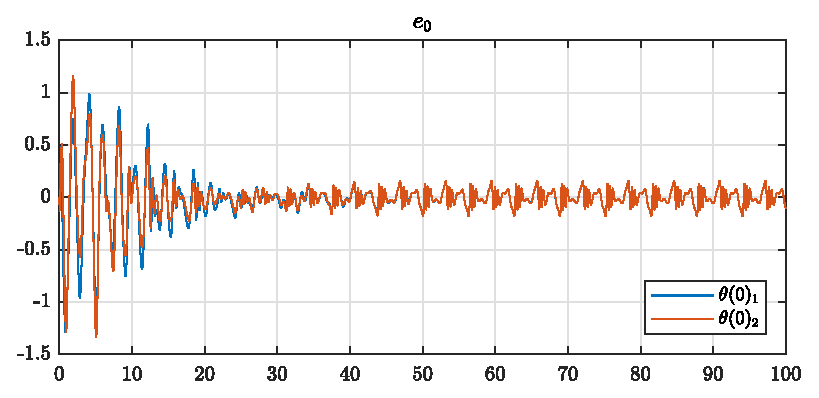
\includegraphics[width=12cm]{figs/e0/sim0_theta0.eps} 
\end{figure}

\begin{figure}[H]
  \centering
  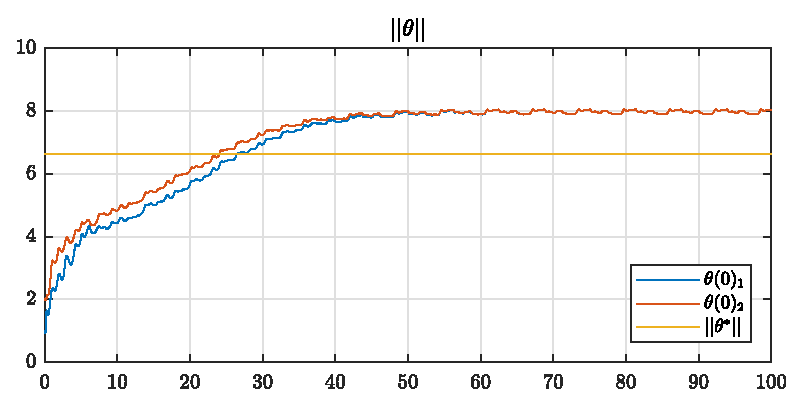
\includegraphics[width=12cm]{figs/modtheta/sim0_theta0.eps} 
\end{figure}

\begin{figure}[H]
  \centering
  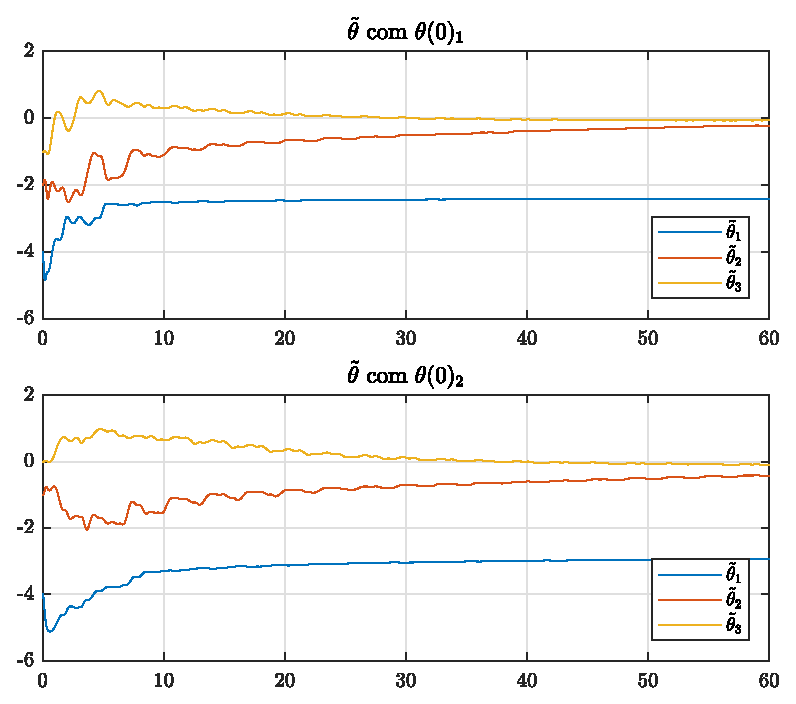
\includegraphics[width=12cm]{figs/tiltheta/sim0_theta0.eps} 
\end{figure}

\begin{figure}[H]
  \centering
  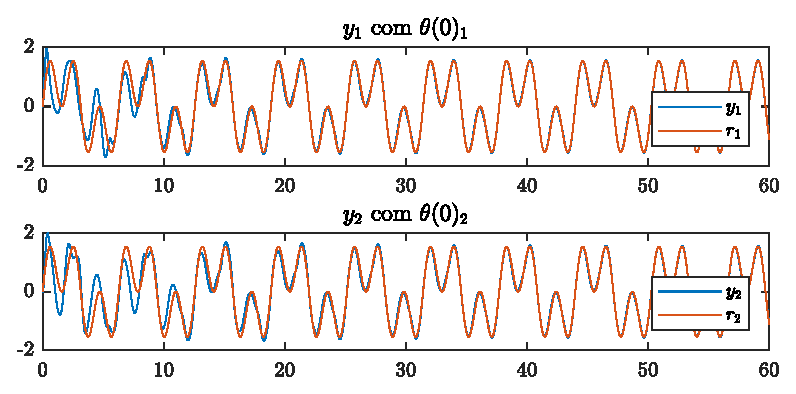
\includegraphics[width=12cm]{figs/y/sim0_theta0.eps} 
\end{figure}

\textbf{\underline{Simula��o 1.2}: $y(0)$}
%
\begin{align*}
  y &= \frac{5}{s^3+3s^2+3s+1}u\,,  &  \theta(0) &= 0 \,,
  & y(0) &=  \HI{0} \, \textrm{e} \, \HI{3} \,, & \Gamma &= 0.5 \\ y_r &= \textrm{sin}(t) + \textrm{sin}(3t) \, & k &= [3
  \quad 3 \quad 3].
\end{align*}

\begin{figure}[H]
  \centering
  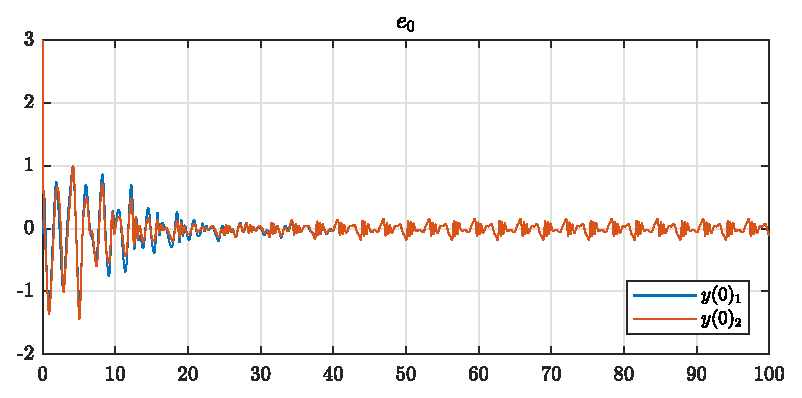
\includegraphics[width=12cm]{figs/e0/sim0_y0.eps} 
\end{figure}

\begin{figure}[H]
  \centering
  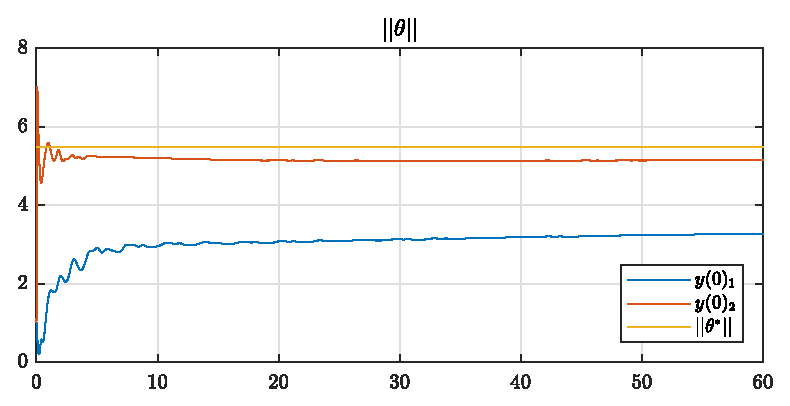
\includegraphics[width=12cm]{figs/modtheta/sim0_y0.eps} 
\end{figure}

\begin{figure}[H]
  \centering
  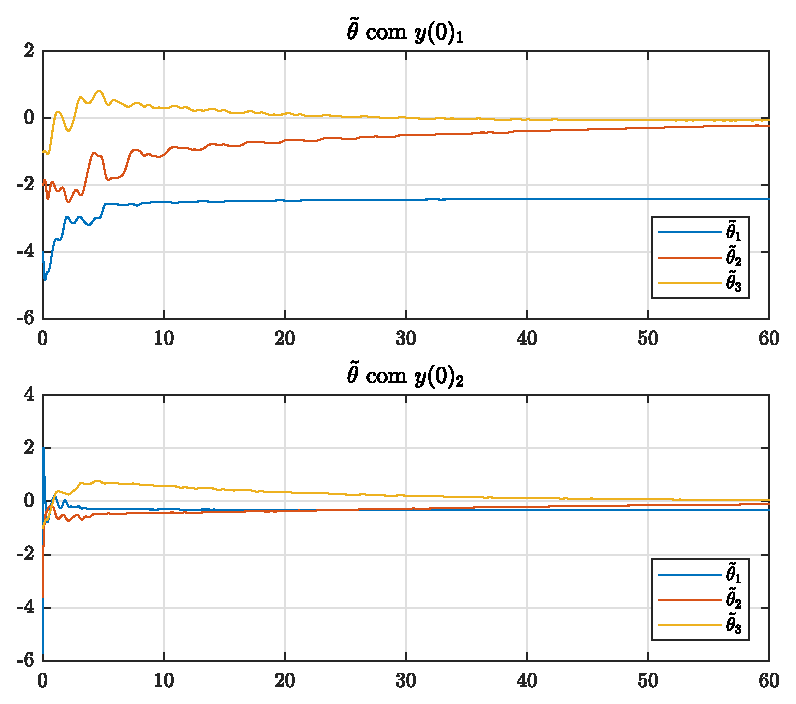
\includegraphics[width=12cm]{figs/tiltheta/sim0_y0.eps} 
\end{figure}

\begin{figure}[H]
  \centering
  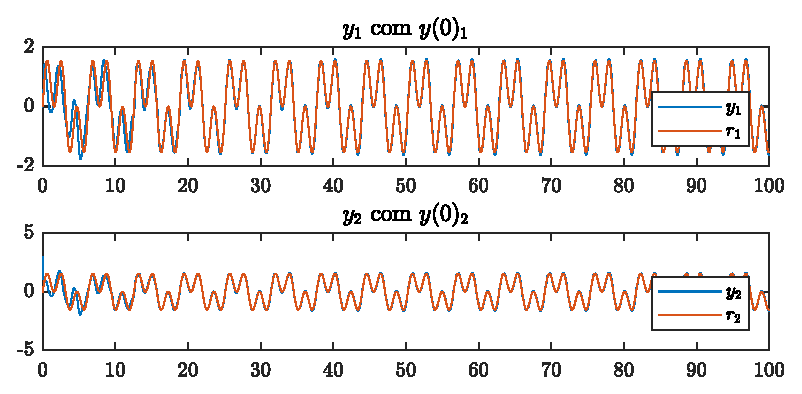
\includegraphics[width=12cm]{figs/y/sim0_y0.eps} 
\end{figure}

\subsection{Simula��o \#2}

Verificamos o comportamento do sistema para varia��es no par�metro de adapta��o
$\Gamma$.

\bigskip

\begin{align*}
  y &= \frac{5}{s^3+3s^2+3s+1}u\,,  &  \theta(0) &= 0 \,,
  & y(0) &=  0 \,, & \Gamma &= \HI{0.1} \, \textrm{e} \, \HI{0.5} \,, \\ y_r &=
  \textrm{sin}(t) + \textrm{sin}(3t) \, & k &= [3 \quad 3 \quad 3].
\end{align*}

\begin{figure}[H]
  \centering
  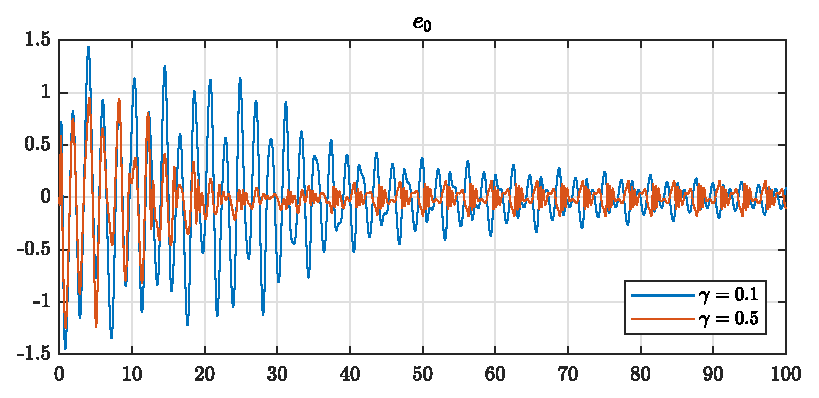
\includegraphics[width=12cm]{figs/e0/sim0_gamma01gamma05.eps} 
\end{figure}

\begin{figure}[H]
  \centering
  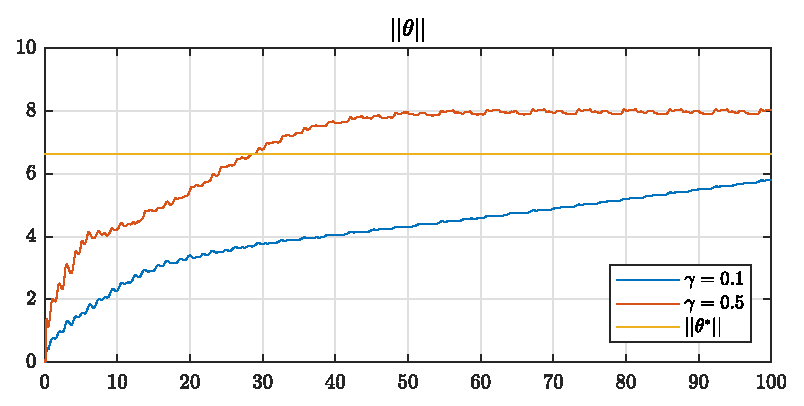
\includegraphics[width=12cm]{figs/modtheta/sim0_gamma01gamma05.eps} 
\end{figure}

\begin{figure}[H]
  \centering
  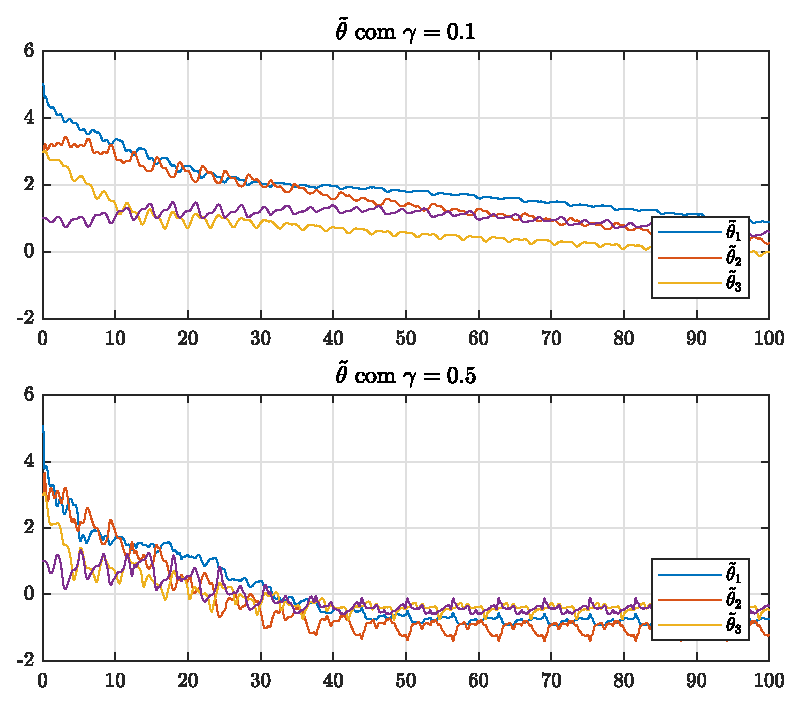
\includegraphics[width=12cm]{figs/tiltheta/sim0_gamma01gamma05.eps} 
\end{figure}

\begin{figure}[H]
  \centering
  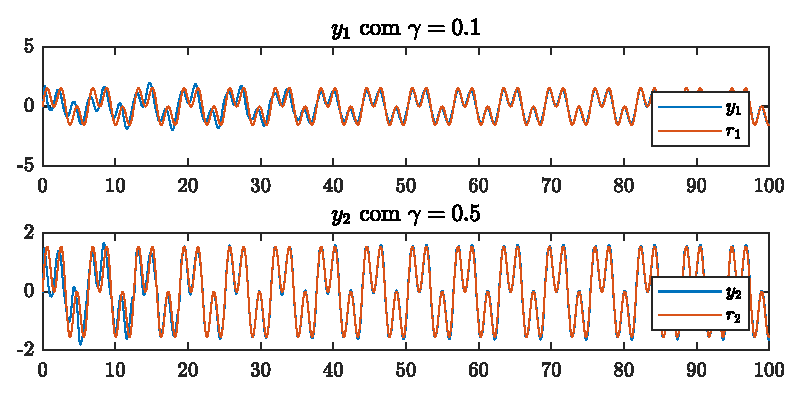
\includegraphics[width=12cm]{figs/y/sim0_gamma01gamma05.eps} 
\end{figure}

\subsection{Simula��o \#3}

Verificamos o comportamento do sistema para varia��es na planta e modelo.

\bigskip

\textbf{\underline{Simula��o 3.1}: planta}
%
\begin{align*}
  y &= \HI{$\frac{5}{s^3+3s^2+3s+1}$}u\, \textrm{e} \,
  \HI{$\frac{5}{s^3-3s^2-3s+1}$}u, & \theta(0) &= 0 \,, & y(0) &=  0 \,, &
  \Gamma &= 0.5 \\ y_r &= \textrm{sin}(t) + \textrm{sin}(3t) \,
  & k &= [3 \quad 3 \quad 3].
\end{align*}

\begin{figure}[H] 
  \centering
  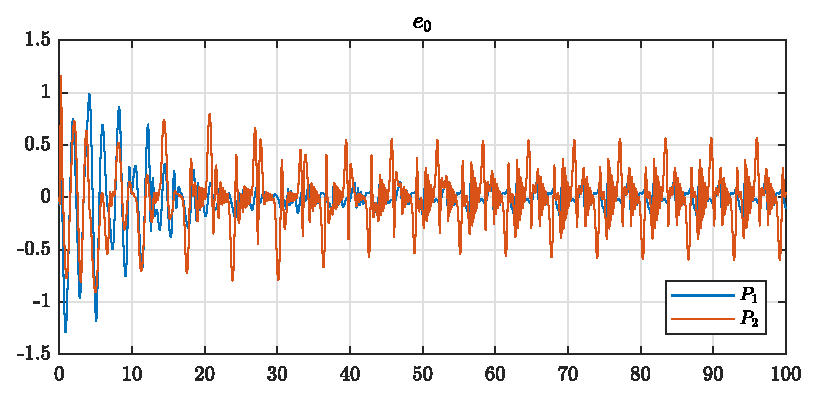
\includegraphics[width=12cm]{figs/e0/sim0_P1P2.eps} 
\end{figure}

\begin{figure}[H]
  \centering
  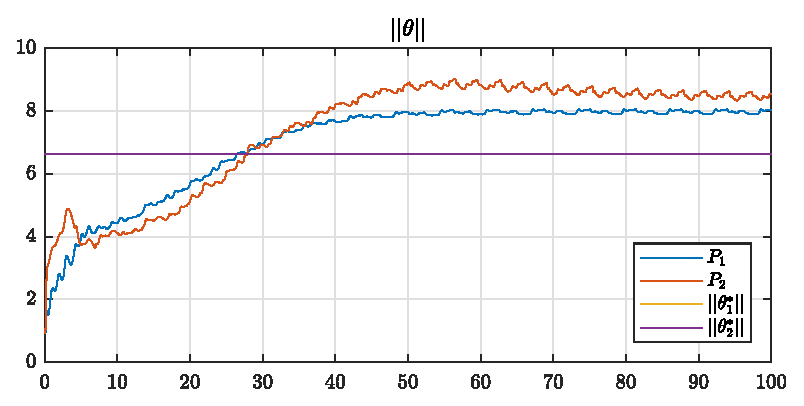
\includegraphics[width=12cm]{figs/modtheta/sim0_P1P2.eps} 
\end{figure}

\begin{figure}[H]
  \centering
  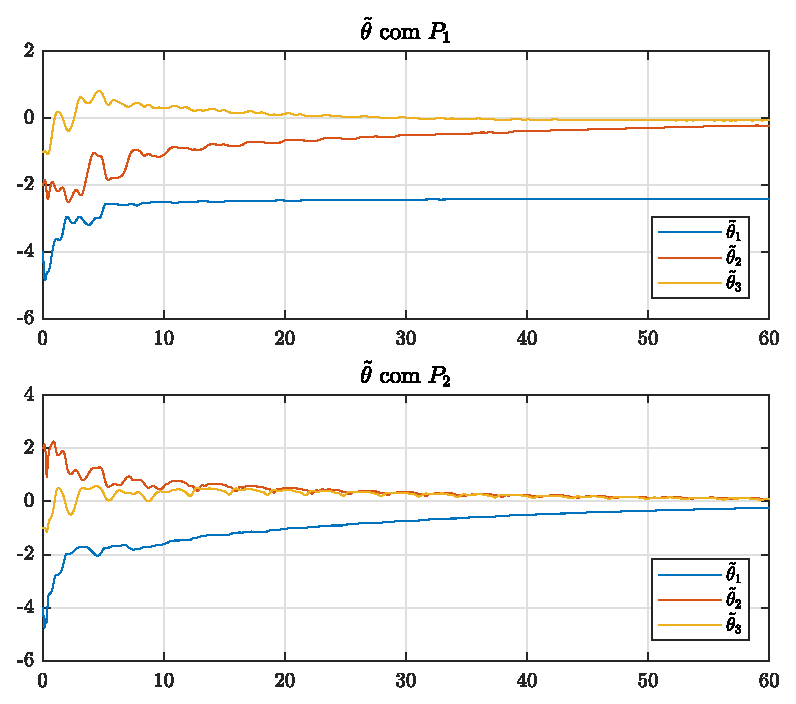
\includegraphics[width=12cm]{figs/tiltheta/sim0_P1P2.eps} 
\end{figure}

\begin{figure}[H]
  \centering
  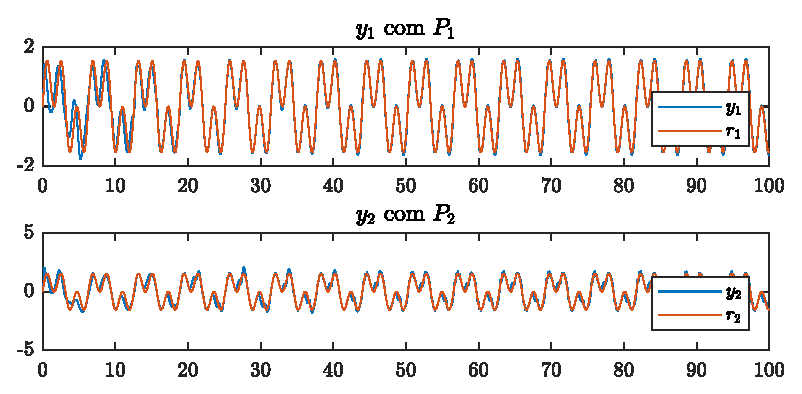
\includegraphics[width=12cm]{figs/y/sim0_P1P2.eps} 
\end{figure}

\textbf{\underline{Simula��o 3.2}: modelo}
%
\begin{align*}
  y &= \frac{5}{s^3+3s^2+3s+1}u\, &  \theta(0) &=
  0 \,, & y(0) &=  0 \,, & \Gamma &= 0.5 \,, \\ y_r &= \HI{$\textrm{sin}(t) +
  \textrm{sin}(3t)$} \, \textrm{e} \, \HI{$\textrm{sin}(t) + \textrm{2sin}(5t)$}
  .
\end{align*}
 
\begin{figure}[H]
  \centering
  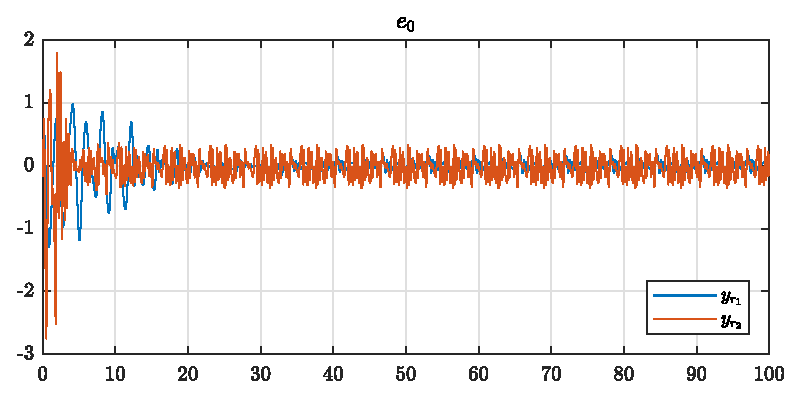
\includegraphics[width=12cm]{figs/e0/sim0_yr1yr2.eps} 
\end{figure}

\begin{figure}[H]
  \centering
  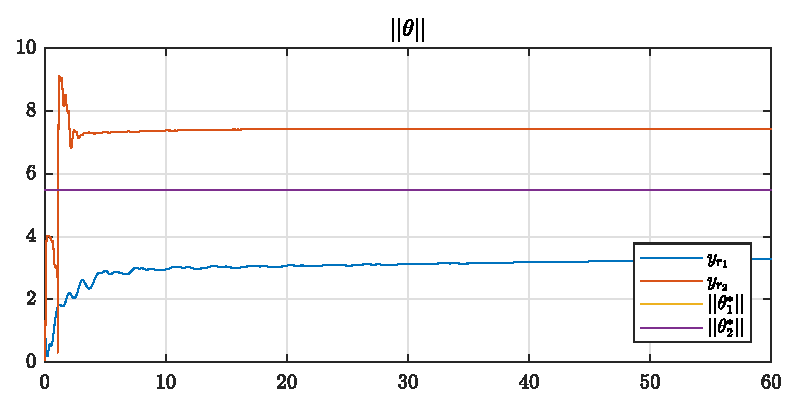
\includegraphics[width=12cm]{figs/modtheta/sim0_yr1yr2.eps} 
\end{figure}

\begin{figure}[H]
  \centering
  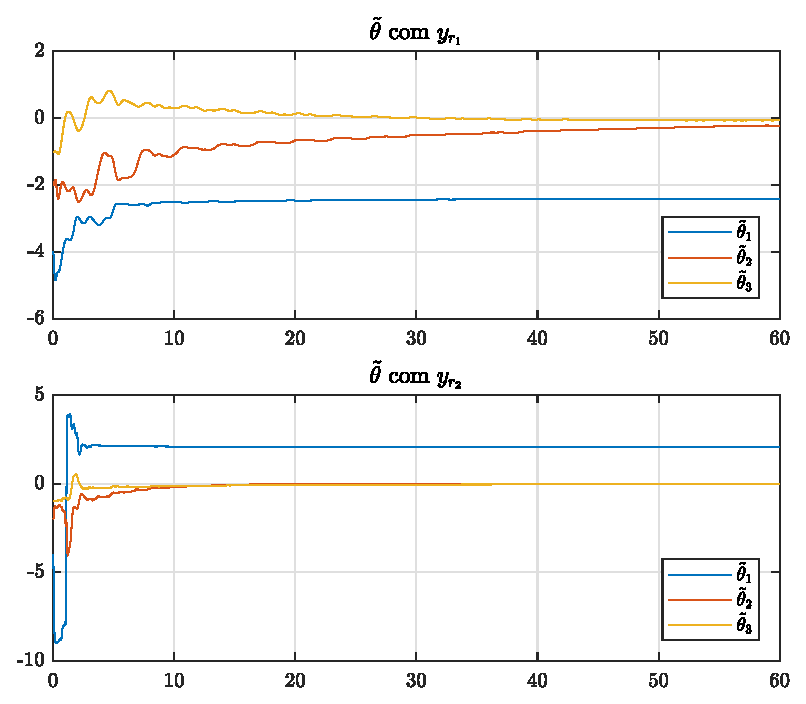
\includegraphics[width=12cm]{figs/tiltheta/sim0_yr1yr2.eps} 
\end{figure}

\begin{figure}[H]
  \centering
  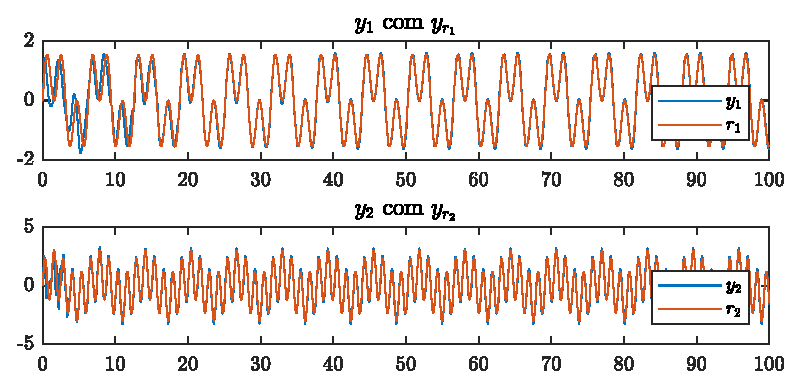
\includegraphics[width=12cm]{figs/y/sim0_yr1yr2.eps} 
\end{figure} \newpage
%---------------------------------------------------------------------
\section{Discuss�o}

Conforme aumentamos a ordem do Backstepping, as derivadas parciais crescem em
grande complexidade, o que requer grande trabalho manual para otimizar o
algoritmo. Al�m disso, o aumento do n�mero de multiplica��es e de novos termos
impede que a simula��o seja r�pida. Verificou-se tamb�m a necessidade da
diminui��o do ganho de adapta��o, se comparado com outros agoritmos como o MRAC,
devido �s multiplica��es e poss�vel overflow num�rico.

A \textbf{simula��o \#1} testou o sistema para condi��es iniciais n�o nulas
tanto dos par�metros $\theta$, quando do sistema $y(0)$. Observou-se a
converg�ncia do erro $e_0$ para zero. Os par�metros convergiram para valores
pr�ximos aos valores esperados.

A \textbf{simula��o \#2} testou o sistema para diferentes valores de
ganho de adapta��o: $\Gamma = 0.1$ e $\Gamma = 0.5$. Para o maior valor,
$\Gamma = 0.5$, o sistema convergiu mais rapidamente, com menor erro, por�m com
maiores oscila��es. Observou-se overflow num�rico para valores $\Gamma > 10$.

A \textbf{simula��o \#3.1} testou o algoritmo para diferentes sistemas,
modelos de tranfer�ncia: $Y/U = \frac{5}{s^3+3s^2+3s+1}$ e $Y/U =
\frac{5}{s^3-3s^2-3s+1}$. Para a planta inst�vel, o algoritmo leva muito tempo
para convergir e as oscila��es s�o maiores.

A \textbf{simula��o \#3.2} testou o algoritmo para diferentes entradas: $r_1 =
\text{sin}(t) + \text{sin}(3t)$ e $r_2 = \text{sin}(t) + 2\text{sin}(5t)$.
Apesar de a entrada de alta frequ�ncia exigir mais do sistema, mostrando maior
lentid�o para a converg�ncia, os par�metros convergiram mais rapidamente.

 
%---------------------------------------------------------------------
%\bibliographystyle{agsm}
%\bibliography{bib,coe736}

%---------------------------------------------------------------------
\end{document}
